\documentclass[11pt]{article}
 
\usepackage[top=0.75in, bottom=1.25in, left=1in, right=1in]{geometry} 
\usepackage{amsmath,amsthm,amssymb} %this is THE math package
\usepackage{mathtools}
\usepackage{tikz}
\usepackage{graphicx}
\usepackage{fancybox}
\usepackage{hyperref}
\usepackage{varwidth}
\usepackage{mdframed}
\usepackage{mathrsfs}
\usepackage[most]{tcolorbox}
%------------------------
%Fonts I use, uncomment if you like to use them.
%The first is the general font, and the second a math font
\usepackage{mathpazo}
\usepackage{eulervm}
\usepackage{graphicx}
\graphicspath{ {./images/} }


%------------------------
%This is so that we have standard fonts for the double-stroked symbols
%for reals, naturals etc. regardless of what font you use.
%Don't comment
\AtBeginDocument{
  \DeclareSymbolFont{AMSb}{U}{msb}{m}{n}
  \DeclareSymbolFontAlphabet{\mathbb}{AMSb}}
%------------------------

%----------------------------------------------
%User-defined environments
%Commented because we're not using them in this document
%The only uncommented ones are the Problem and Solution environment

% \newenvironment{theorem}[2][Theorem]{\begin{trivlist}
% \item[\hskip \labelsep {\bfseries #1}\hskip \labelsep {\bfseries #2.}]}{\end{trivlist}}
% \newenvironment{lemma}[2][Lemma]{\begin{trivlist}
% \item[\hskip \labelsep {\bfseries #1}\hskip \labelsep {\bfseries #2.}]}{\end{trivlist}}
% \newenvironment{exercise}[2][Exercise]{\begin{trivlist}
% \item[\hskip \labelsep {\bfseries #1}\hskip \labelsep {\bfseries #2.}]}{\end{trivlist}}
% \newenvironment{question}[2][Question]{\begin{trivlist}
% \item[\hskip \labelsep {\bfseries #1}\hskip \labelsep {\bfseries #2.}]}{\end{trivlist}}
% \newenvironment{corollary}[2][Corollary]{\begin{trivlist}
% \item[\hskip \labelsep {\bfseries #1}\hskip \labelsep {\bfseries #2.}]}{\end{trivlist}}
\newenvironment{problem}[2][Problem\!]{\begin{trivlist}
\item[\hskip \labelsep {\bfseries #1}\hskip \labelsep {\bfseries #2}]}{\end{trivlist}}
%\newenvironment{sub-problem}[2][]{\begin{trivlist}
%\item[\hskip \labelsep {\bfseries #1}\hskip \labelsep {\bfseries #2}]}{\end{trivlist}}
\newenvironment{solution}{\begin{proof}[\textbf{\textit{Solution}}] }{\end{proof}}
%----------------------------------------------

%----------------------------
%User-defined notations
\newcommand{\zz}{\mathbb Z}   %blackboard bold Z
\newcommand{\qq}{\mathbb Q}   %blackboard bold Q
\newcommand{\ff}{\mathbb F}   %blackboard bold F
\newcommand{\rr}{\mathbb R}   %blackboard bold R
\newcommand{\nn}{\mathbb N}   %blackboard bold N
\newcommand{\cc}{\mathbb C}   %blackboard bold C
\newcommand{\af}{\mathbb A}   %blackboard bold A
\newcommand{\pp}{\mathbb P}   %blackboard bold P
\newcommand{\id}{\operatorname{id}} %for identity map
\newcommand{\im}{\operatorname{im}} %for image of a function
\newcommand{\dom}{\operatorname{dom}} %for domain of a function
\newcommand{\cat}[1]{\mathscr{#1}}   %calligraphic category
\newcommand{\abs}[1]{\left\lvert#1\right\rvert} %for absolute value
\newcommand{\norm}[1]{\left\lVert#1\right\rVert} %for norm
\newcommand{\modar}[1]{\text{ mod }{#1}} %for modular arithmetic
\newcommand{\set}[1]{\left\{#1\right\}} %for set
\newcommand{\setp}[2]{\left\{#1\ \middle|\ #2\right\}} %for set with a property
\newcommand{\card}[1]{\#\,{#1}} %for cardinality of a set
\newcommand\m[1]{\begin{pmatrix}#1\end{pmatrix}} 

%Re-defined notations
\renewcommand{\epsilon}{\varepsilon}
\renewcommand{\phi}{\varphi}
\renewcommand{\emptyset}{\varnothing}
\renewcommand{\geq}{\geqslant}
\renewcommand{\leq}{\leqslant}
\renewcommand{\Re}{\operatorname{Re}}
\renewcommand{\Im}{\operatorname{Im}}
%----------------------------

\allowdisplaybreaks
 
 
\begin{document}
 
\title{12/03 Resubmission}
\author{Kevin Guillen\\[0.5em]
MATH 101 | Problem Solving | Fall 2021}
\date{} 
\maketitle

%Use \[...\] instead of $$...$$

\begin{tcolorbox}
    \begin{problem}{10/8 | OC | 30. }
        Chose any $(n+1)$ element subset of $\set{1,2,\dots, 2n}$. Show that this subset contains two elements which are relatively prime. 
    \end{problem}
\end{tcolorbox}
\begin{proof}
    Let $S$ denote the set $\set{1,2,\dots,2n}$. To prove this we will use the pigeon hole principle and the fact that two neighboring numbers are relatively prime. Our "pigeonholes" in this case will be a list of n+1 numbers in ascending order.  The max amount of numbers that can be chosen from $\set{1,2, \dots , 2n}$ such that no numbers are relatively prime would be $n$, because consecutive numbers in our list will have a difference of at least 2. Since we are choosing $n+1$ numbers though 1 number in our list will have to have a difference of 1 with the number next to it in the list. As a result these two numbers will be relatively prime. 
\end{proof}

\begin{tcolorbox}
    \begin{problem}{10/11 IC (44.)} 
        The numbers $1,2,\dots, 50$ are written on the blackboard. Then two numbers $a$ and $b$ are chosen and replaced by the single number $\abs{a-b}$. After 49 operations a single number is left. Prove that it is odd. 
    \end{problem}
\end{tcolorbox}

\begin{proof}
    If we have the numbers $1,2,\dots, 50$ that means half of them are even and half are odd. In other words we have 25 even numbers and 25 odd numbers. We know after 49 operations we will have a single number left. To determine if it is odd or even let's look at the 3 scenarios when taking the differences of even and odd numbers.
    \begin{alignat*}{2}
        &\text{Two even numbers: } 2k - 2l &&= 2(k-l) \\
        &\text{Odd and even numbers: } 2k + 1 - 2l &&= 2(k-l) + 1 \\
        &\text{Two odd numbers: } 2k + 1 - (2l + 1) &&= 2(k-l)
    \end{alignat*}

    Since in the set of number $\set{1,2, 3, \dots, 50}$. Half of these numbers are odd, more specifically there are an odd number of odd numbers. This means our last number will have to be odd because the only way to remove odd numbers when summing is to add two of them together, meaning we would have needed an even amount.
\end{proof}
\newpage

\begin{tcolorbox}
    \begin{problem}{10/11 IC (46.)} Seven quarters are initially all heads up. On a single move you can choose any four and turn them over (change heads to tails and tails to heads). Is it possible to obtain all tails up after a sequence of such moves?
    \end{problem}
\end{tcolorbox}
\begin{solution}
    This is impossible, we will show this by showing the number of heads will always be odd and the number of tails will always be even. This is important since the state of the coins before the "winning" move would have to be where we have 4 heads and 3 tails, since we'd simply flip all 4 heads to tails.
    Consider this though, after the first move we will have 3H and 4T.

    We have (2k + 1) heads and (2n) tails. If we flip 1 heads and 3 tails this changes the coin state by adding 2 heads and removing 2 tails, (2(k+1) + 1) heads and (2(n-1)) tails.

    If we flip 2 heads and 2 tails this does nothing.

    If we flip 3 heads to 1 tails this changes the coin state by adding 2 tails and removing 2 heads, (2(k-1) + 1) heads and (2(n + 1)). 

    If we can flip 4 tails to heads that would give us (2(k + 2) + 1) heads which is still odd.

    If we can flip 4 heads to tails that would give us (2(k-2) + 1) heads which is also still odd.

    Since we can't obtain a state of having an even number of heads, we can never have a sequence that results in all tails up.
\end{solution}

\begin{tcolorbox}
    \begin{problem}{10/13 IC (50.)} 
        Every room in a house has an even number of doors. Prove that there are an even number of entrance doors to the house. 
    \end{problem}
\end{tcolorbox}
\begin{solution}
    Let each room in the house be a vertex and outside be a vertex as well. All we have to show now is that this graph can't have exactly one vertex of odd degree. By the handshaking lemma there does not exist any such graph. So we have an even number of vertices which have odd degree. So connecting each adjacent door by an edge each entrance door has odd degree, therefore by handshaking lemma we have an even number of entrance doors. 
\end{solution}

\begin{tcolorbox}
    \begin{problem} {OC | 11/01 | 68}
        Imagine an $n \times n$ chessboard. How many ways is it possible to choose four squares, no three in the same row or columns which are the vertices of a rectangle?
    \end{problem}
\end{tcolorbox}
\begin{proof}
    If we have an $n\times n$ chessboard that means we have $n$ columns and $n$ rows. We can treat each row and column as sides of a rectangles. If we choose 2 unique vertical lines and 2 unique horizontal lines their intersections will generate a rectangle. There are n choose 2 ways to pick our horizontal lines, and n choose 2 ways to pick our vertical lines This means for an $n \times n$ chessboard we have, 
    \[\binom{n}{2}\binom{n}{2}\]
    rectangles

\end{proof}
\newpage
\begin{tcolorbox}
    \begin{problem} {OC | 11/10 | 86.}
        Prove that there are no positive integers $x$, $y$ such that $x+y$, $2x + y$, and $x + 2y$ are squares. 
    \end{problem}
\end{tcolorbox}
\begin{proof}
    Assuming this were to be true, then for integers $a$, $b$, and $c$ we have,
    \begin{align*}
        x+y &= a^{2} \\
        2x+y &= b^{2} \\
        x + 2y &= c^{2}
    \end{align*}
    Using the 2nd equation to solve for $y$ we get, $y = b^{2} -2x$. Plugging this into the 1st equation we get, $x = b^{2} - a^{2}$. Using the 1st equation to solve for $x$ we get, $x = a^{2} -y$. Pluggin this into the 2nd equation we get $y = 2a^{2} -b^{2}$.

    Now plugging in these value into the 3rd equation, we get,
    \begin{align*}
        a^{2}-y + 4a^{2} -2b^{2} &= c^{2} \\
        3a^{2} &= b^{2} + c^{2}
    \end{align*}

    Thus there is only integer solutions if this diophantine equation holds. We know any integers squared mod 4 will have values 0 or 1. Therfore $b^{2} + c^{2} \in \set{0,1,2}$, and $3a^{2}\in \set{0,3}$. This together means we must have $3a^{2} \equiv 0 \text{ mod } 4$ and $(b^{2} + c^{2}) \equiv 0 \text{ mod }4$. Meaning $a$ is even and is of the form $a = 2k$, also means that $b$ and $c$ are even and of the form $b = 2l$ and $c = 2n$. Plugging this back into the equation we get,
    \begin{align*}
        12k^{2} & = 4l^{2} + 4n^{2}.
    \end{align*}

    This means there has to be a solution for $k$, $l$, and $n$. But this can be since $k + l + n < a + b + c$. Therefore there is no integers $x$ and $y$ such that $x +y$, $2x +y$, and $x + 2y$ are squares.
\end{proof}

\begin{tcolorbox}
    \begin{problem} {OC | 11/10 | 88.}
        Prove that there does not exist a natural number $n$ such that $n(n+1)$ is a perfect square.
    \end{problem}
\end{tcolorbox}
\begin{proof}
    Assume $n(n+1)$ is indeed a perfect square. That means it can expressed as, $n(n+1)= k^{2}$ for some $k \in \zz$. Consider the following though,
    \begin{align*}
        n(n+1) &= k^{2} \\
        n^{2} + n &= k^{2} \\
        n^{2} + k^{2} &= -n \\
        (n+k)(n-k) &= -n
    \end{align*}

    We know $k > n$ meaning, $n +k  > n$. We have a contradiction now then since the equation implies $(n+k) \mid -n$ which is impossible since $n-k \in \zz$. Therefore there exists no natural number $n$ such that $n(n+1)$ is a perfect square. 
\end{proof}
\newpage
\begin{tcolorbox}
    \begin{problem} {IC | 11/01 | 109.}
        How many solutions in natural numbers are there to the equation $a + b + c + d = 12$ where $a$ and $b$ are odd, and $c,d$ are arbitrary natural numbers?
    \end{problem}
\end{tcolorbox}
\begin{proof}
    We can solve this using generating functions and looking at the coefficient of $x^{12}$ for,
    \begin{align*}
        (x + x^{3} + x^{5} + x^{7} + x^{9})^{2}(x + x^{2} + \dots + x^{9})^{2}
    \end{align*}
    We are squaring the first term since that represents our 2 odd numbers and the second term is squared representing the arbitrary natural numbers. Which is why the first term has odd powers and the second term has every power up to 9. After calculations we will have the coefficient of $x^{12}$ to be 55. Meaning there is 55 solutions.
    
\end{proof}

\begin{tcolorbox}
    \begin{problem} {IC | 11/15 | 151.}
        Is it possible for a triangle to have altitudes equal to 6, 10, and 20?
    \end{problem}
\end{tcolorbox}
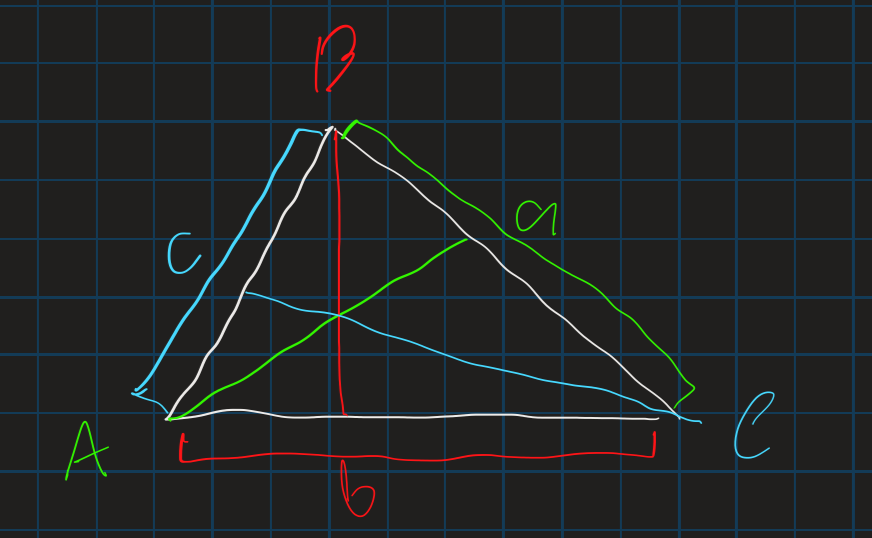
\includegraphics[scale=.5]{prob2}
\begin{proof}
    Consider the area of the triangle drawn above. It will be the following,
    \[A = \frac{6}{2}a = \frac{10}{2}b = \frac{20}{2}c.\]

    Which gives us the following equations,
    \begin{align*}
        a &= \frac{1}{3}A \\
        b &= \frac{1}{5}A \\
        c &= \frac{1}{10}A
    \end{align*}

    Recall though by the triangle inequality we have that $a < b + c$, we see through the following though,
    \begin{align*}
        a &< b + c \\
        \frac{10}{30}A &< \frac{6}{30}A + \frac{3}{10}A = \frac{9}{10}A
    \end{align*}
    that if our altitudes were 6, 10 and 20, that would imply $\dfrac{10}{30}A < \dfrac{9}{10}A$ which is a contradiction. Therefore there can not be a triangle with those given altitudes. 
\end{proof}







\newpage
\begin{tcolorbox}
    \begin{problem} {OC | 11/24 | PP21}
        A class with $2N$ students score $1,2, \dots, 10$. Each of these score occurred at least once, the average was 7.4. Show that the group can be divided into two groups such that the average is 7.4.
    \end{problem}
\end{tcolorbox}
\begin{proof}
    First let us consider the sum of all the scores which will simply be $S= x_1 + x_2 + \dots + x_{2N} = (7.4)2N$. Which we can express as,
    \[S = \frac{5}{5}(7.4)2N = \frac{74N}{5}.\]
    This gives us that 5 divides $N$ and that the total sum is even. Now let $x_1, x_2, \dots x_{2N}$ be the sequence of scores in ascending order. Next let us define $y_k = x_{2k} - x_{2k -1}$. We know the $y_k$ will either be 1 or 0, this is because for any two consecutive scores we have that they will be equal or 1 apart and since every score occurs at least once. Let $S'$ be the sum of $y_1 + y_2 + \dots y_N$. Because $S$ is even, $S'$ must also be even. This means there is some $m < N$, such that,
    \[y_1 + y_2 + \dots + y_m = \frac{S'}{2}.\]
    Now if we consider the scores of $x_2,x_4, \dots x_{2m}, x_{2m+1} , \dots,  x_{2N -1 } $ and their sum denoted by $T$,
    \begin{align*}
        T &=x_2 + x_4 + \dots + x_{2m} + x_{2m + 1} + \dots + x_{2N - 1} && \left(y_k = x_{2k} - x_{2k -1}\right) \\
        T &=(y_1 + x_1 ) + \dots (y_m + x_{2m - 1}) + x_{2m + 1} + \dots + x_{2N-1} \\
        T &=(y_1 + y_2 + \dots + y_m) + (x_1 + x_3 + \dots x_{2m+1} + \dots + x_{2N-1}) &&  \left(y_1 + \dots + y_m = \frac{S'}{2}\right) \\
        T &=\frac{1}{2}(S' + 2x_1 + 2x_3 + \dots + x_{2N-1}) &&  \left(y_1 + y_2 + \dots + y_N = S'\right) \\
        T &=\frac{1}{2} (((y_1 + x_1) +  \dots + (y_N + x_{2N - 1})) + (x_1 + x_3 + \dots + x_{2N-1})) && \left(y_k = x_{2k} - x_{2k -1}\right)\\
        T &=\frac{1}{2} (x_2 + \dots + x_{2N} + x_1 + x_3 \dots x_{2N-1}) \\
        T &= \frac{1}{2}(x_1 + x_2 + \dots + x_{2N}) \\
        T &=\frac{1}{2} S
    \end{align*}

    But $\dfrac{1}{2}S$ is simply $7.4 \cdot N$. Thus the average of this collection of student scores is $7.4$ and as a consequence the average of the student's scores not in this group must also be $7.4$. Meaning we have broken the students into two groups where the average is still the same. 
\end{proof}

\end{document}
